\documentclass[11pt,a4paper,twocolumn]{article}
\usepackage[cm]{fullpage}
\usepackage[compact]{titlesec}
\usepackage{mathtools}
\usepackage{graphicx}
\usepackage[hidelinks]{hyperref}
\usepackage[group-separator={,}]{siunitx}
\begin{document}
\title{Stochastic Simulation of Morphogen Gradients During Drosophila Melanogaster Embryogenesis}
\author{Maxwell Conway}
\date{}
\maketitle
\section{Introduction}
The topic investigated in this project was Drosophila Embryogenesis, specifically the interaction of the morphogens Bicoid, Caudal, Nanos and Hunchback. This topic, while a highly studied system, had not been modelled stochastically before. We built a total of 105 different models using the Smoldyn~\cite{Andrews2010} particle based simulation suite, covering 20 different species and 38 reactions, over development cycles 1-13. Results were validated against quantitative data from the Flyex database~\cite{Pisarev2009}, showing good agreement, which both supports the accuracy of our model and the deterministic models on which it is based. 

\section{Species, Models and Results}
The first species studied was Bicoid, due to its extensive characterization. After creating and validating several models of just the Bicoid gradient, we moved on to the other morphogens.
\subsection{Bicoid}
Our basic model~\cite{Grimm2010} for Bicoid was a fixed region of mRNA in the anterior of the cell, which was translated to bicoid protein at a constant rate; this protein degraded at a constant rate of \(0.0003s^{-1}\). Diffusion rates of \(0.3s^{-1}\), \(4s^{-1}\) and \(7.4s^{-1}\) were used, all literature derived. This produced a stable gradient by cycle 13 at all diffusion rates, but  \(4s^{-1}\) provided the best fit to Flyex data.  We also experimented with refinements of this model (see figure~\ref{fig:bcd-grads}):
\begin{description}
\item[Increasing Translation rate~\cite{Holloway2011}:]
This model had the Bicoid mRNA translation rate increasing throughout the duration of development due to polyadenylation. In our simulations it had not reached stability by cycle 13, but was changing very slowly.
\item[mRNA transport:]
Here we simulated the action of cytoskeletal mRNA transport by starting directed diffusion of Bicoid mRNA towards the posterior of the cell at fertilization and at 1,620 seconds into the simulation, but with this mRNA confined to near the cell membrane~\cite{Spirov2009}. Obviously this acted the same as the basic model until the start of diffusion, but after this point produced a flatter gradient, with a peak slightly further from the anterior, especially when mRNA transport had been allowed to proceed from fertilization.
\end{description}

\begin{figure}[h!]
  \centering
    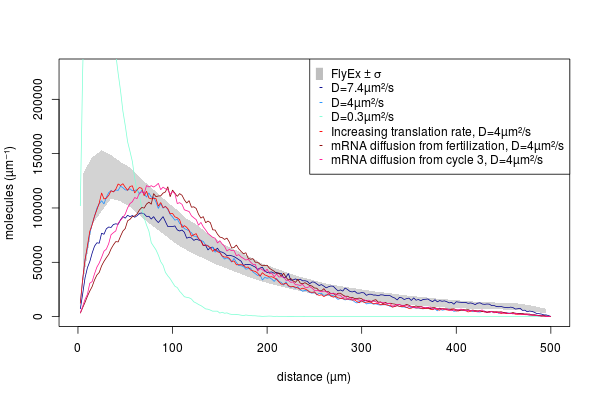
\includegraphics[width=0.5\textwidth]{writeup-bcd-diffusion}
  \caption{Bicoid gradients. D is diffusion coefficient. \label{fig:bcd-grads}}
\end{figure}

\subsection{Caudal}
Caudal mRNA was created in an even distribution throughout the cytoplasm, with constant protein production and decay rates~\cite{Bergmann2007}. However, Bicoid protein could bind to Caudal mRNA to stop transcription, producing a gradient opposite to of Bicoid, peaking in the posterior.

\subsection{Nanos}
Nanos mRNA was created fixed in the posterior of the cell, and created protein in much the same way as Bicoid~\cite{Kugler2009,Bergmann2007}. However, this protein inhibited Bicoid translation~\cite{Little2011}, making the Bicoid gradient steeper in the case where mRNA could diffuse, and causing faster stabilization of the Bicoid gradient in all cases.

\subsection{Hunchback}
The Hunchback model was by far the most complex, but neverthless all rates in it are derived from experimental data. It consists of simple Hunchback transcription and inhibition by Nanos protein, increasing number of nuclei over time (modelled as particles), and 24 reactions to fully model zygotic transcription using 8 different complexes~\cite{Holloway2011}. The simple model of Hunchback inhibition by Nanos fitted the experimentally predicted downwards gradient along the anterior-posterior axis, but the full zygotic transcription model suffered performance issues that meant that, even allowing several days of runtime, noise levels were still too high to assert anything more than a qualitative fit (see figure~\ref{fig:all}).

\begin{figure}[h!]
  \centering
    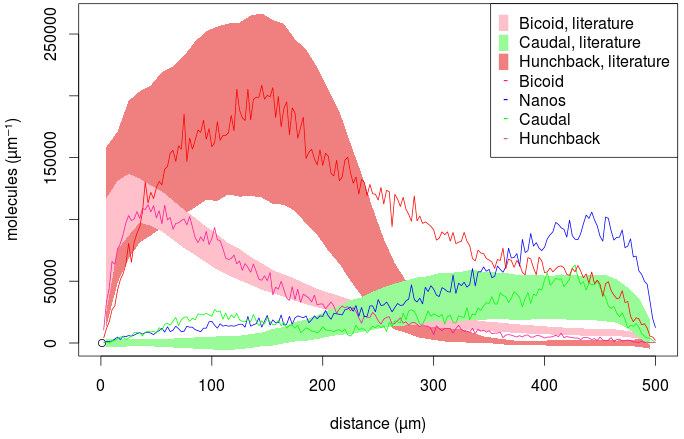
\includegraphics[width=0.5\textwidth]{writeup-all}
  \caption{Gradients for all morphogens. \label{fig:all}}
\end{figure}

\section{Methods}
Some division of labour was used in order to get the best possible result in the time available. My main focus was on the simulation, especially the more technical aspects, and on analysis and presentation of results.

\subsection{Framework}
A data handling framework was built around Smoldyn using Python and the Make build system to allow for many simulations to be run in parallel over extended periods. The first stage to this was parameter processing and insertion. This allowed all models to be stored in a spreadsheet, for easy set up and to streamline creation of new molecules based on existing ones. A Python program processed this spreadsheet to build the Smoldyn files for all of the models listed - far more than could reasonably have been constructed by hand. 

The Make build system was used to schedule simulations. This found all models for which the corresponding results file was out of date or not created yet, and scheduled them for simulation, with the number of concurrent simulations equal to the number of processors available, and new simulations scheduled as old ones were completed. Once all results were up to date, they were automatically copied to a folder for analysis, ensuring a consistent results set.

The Git version control system was used to manage source code and parameter files. This allowed us to roll back unwanted alterations on several occasions, saving significant time. Our full source code is published at \url{git.io/uVrL8g}.

Analysis was conducted in R. Comprehensive use of functions and scripting allowed every graph to be kept up to date and for the effects of parameter changes to be rapidly understood.

\subsection{Accuracy vs Speed}
Most models required some experimentation to find a point at which the desired level of accuracy could be achieved within a reasonable runtime. Time step lengths were tried between \(1s\) and \(10s\), while molecule number scaling factors between \(10^2\) and \(10^4\) were used. 

Ensuring simulation accuracy was especially important in simulations of the behaviour of Bicoid mRNA and protein, since for these literature data was available that allowed for accurate parametrization, so that the simulation could be expected to produce quantitatively accurate output. For this reason, these simulations used a \(1s\) time step to ensure a spatial resolution of \(4\mu m\), based on the equation in the Smoldyn manual~\cite{Andrews2011}. A scaling factor of 100 was used, though in the Bicoid models without inhibition effects, this affected only precision, not accuracy.

In the more complex models, such as those including Hunchback, some quantitative accuracy had to be sacrificed for qualitative results, such as by increasing the time step used. Unfortunately, because the Hunchback models took such a disproportionately long time to run, Camgrid was not able to provide a significant speedup, due to Amdahl’s law. A possible extension to this project would be to move to a GPU Smoldyn implementation, which could provide a speedup of around 130x~\cite{Dematte2010}, enabling one to one simulation of molecules within hours or days.

%\begin{figure}[h!]
% \centering
%    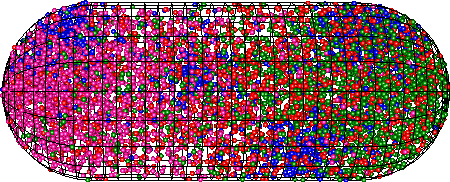
\includegraphics[width=0.5\textwidth]{frame846}
%\caption{an image from during simulation with all 4 morphogens. Molecule count had to be very low}
%\end{figure}

\section{Conclusion}
The best model for Bicoid (the simplest model with a diffusion rate of \(4s^{-1}\)) and Caudal followed the Flyex data well. Since our model is based on literature derived values, this lends significant support to the relatively simple model of Bicoid diffusion that delivered the best results. 

Nanos and Hunchback delivered qualitatively correct results. These would require further experimental data and more computing time in order to quantitatively evaluate.

Detailed results available upon request from \href{mailto:mjc233@cam.ac.uk}{mjc233@cam.ac.uk}.

\nocite{*}
\pagebreak[4]
\bibliographystyle{plain}
\bibliography{drosophila-embryogenesis}
\end{document}